
%% bare_jrnl_compsoc.tex
%% V1.4b
%% 2015/08/26
%% by Michael Shell
%% See:
%% http://www.michaelshell.org/
%% for current contact information.
%%
%% This is a skeleton file demonstrating the use of IEEEtran.cls
%% (requires IEEEtran.cls version 1.8b or later) with an IEEE
%% Computer Society journal paper.
%%
%% Support sites:
%% http://www.michaelshell.org/tex/ieeetran/
%% http://www.ctan.org/pkg/ieeetran
%% and
%% http://www.ieee.org/

%%*************************************************************************
%% Legal Notice:
%% This code is offered as-is without any warranty either expressed or
%% implied; without even the implied warranty of MERCHANTABILITY or
%% FITNESS FOR A PARTICULAR PURPOSE! 
%% User assumes all risk.
%% In no event shall the IEEE or any contributor to this code be liable for
%% any damages or losses, including, but not limited to, incidental,
%% consequential, or any other damages, resulting from the use or misuse
%% of any information contained here.
%%
%% All comments are the opinions of their respective authors and are not
%% necessarily endorsed by the IEEE.
%%
%% This work is distributed under the LaTeX Project Public License (LPPL)
%% ( http://www.latex-project.org/ ) version 1.3, and may be freely used,

\documentclass[10pt,journal, compsoc]{IEEEtran}
%
% If IEEEtran.cls has not been installed into the LaTeX system files,
% manually specify the path to it like:
% \documentclass[10pt,journal,compsoc]{../sty/IEEEtran}





% Some very useful LaTeX packages include:
% (uncomment the ones you want to load)


% *** MISC UTILITY PACKAGES ***
%
%\usepackage{ifpdf}
% Heiko Oberdiek's ifpdf.sty is very useful if you need conditional
% compilation based on whether the output is pdf or dvi.
% usage:
% \ifpdf
%   % pdf code
% \else
%   % dvi code
% \fi
% The latest version of ifpdf.sty can be obtained from:
% http://www.ctan.org/pkg/ifpdf
% Also, note that IEEEtran.cls V1.7 and later provides a builtin
% \ifCLASSINFOpdf conditional that works the same way.
% When switching from latex to pdflatex and vice-versa, the compiler may
% have to be run twice to clear warning/error messages.






% *** CITATION PACKAGES ***
%
\ifCLASSOPTIONcompsoc
  % IEEE Computer Society needs nocompress option
  % requires cite.sty v4.0 or later (November 2003)
  \usepackage[nocompress]{cite}
\else
  % normal IEEE
  \usepackage{cite}
\fi
% cite.sty was written by Donald Arseneau
% V1.6 and later of IEEEtran pre-defines the format of the cite.sty package
% \cite{} output to follow that of the IEEE. Loading the cite package will
% result in citation numbers being automatically sorted and properly
% "compressed/ranged". e.g., [1], [9], [2], [7], [5], [6] without using
% cite.sty will become [1], [2], [5]--[7], [9] using cite.sty. cite.sty's
% \cite will automatically add leading space, if needed. Use cite.sty's
% noadjust option (cite.sty V3.8 and later) if you want to turn this off
% such as if a citation ever needs to be enclosed in parenthesis.
% cite.sty is already installed on most LaTeX systems. Be sure and use
% version 5.0 (2009-03-20) and later if using hyperref.sty.
% The latest version can be obtained at:
% http://www.ctan.org/pkg/cite
% The documentation is contained in the cite.sty file itself.
%
% Note that some packages require special options to format as the Computer
% Society requires. In particular, Computer Society  papers do not use
% compressed citation ranges as is done in typical IEEE papers
% (e.g., [1]-[4]). Instead, they list every citation separately in order
% (e.g., [1], [2], [3], [4]). To get the latter we need to load the cite
% package with the nocompress option which is supported by cite.sty v4.0
% and later. Note also the use of a CLASSOPTION conditional provided by
% IEEEtran.cls V1.7 and later.





% *** GRAPHICS RELATED PACKAGES ***
%
\ifCLASSINFOpdf
  % \usepackage[pdftex]{graphicx}
  % declare the path(s) where your graphic files are
  % \graphicspath{{../pdf/}{../jpeg/}}
  % and their extensions so you won't have to specify these with
  % every instance of \includegraphics
  % \DeclareGraphicsExtensions{.pdf,.jpeg,.png}
\else
  % or other class option (dvipsone, dvipdf, if not using dvips). graphicx
  % will default to the driver specified in the system graphics.cfg if no
  % driver is specified.
  % \usepackage[dvips]{graphicx}
  % declare the path(s) where your graphic files are
  % \graphicspath{{../eps/}}
  % and their extensions so you won't have to specify these with
  % every instance of \includegraphics
  % \DeclareGraphicsExtensions{.eps}
\fi
% graphicx was written by David Carlisle and Sebastian Rahtz. It is
% required if you want graphics, photos, etc. graphicx.sty is already
% installed on most LaTeX systems. The latest version and documentation
% can be obtained at: 
% http://www.ctan.org/pkg/graphicx
% Another good source of documentation is "Using Imported Graphics in
% LaTeX2e" by Keith Reckdahl which can be found at:
% http://www.ctan.org/pkg/epslatex
%
% latex, and pdflatex in dvi mode, support graphics in encapsulated
% postscript (.eps) format. pdflatex in pdf mode supports graphics
% in .pdf, .jpeg, .png and .mps (metapost) formats. Users should ensure
% that all non-photo figures use a vector format (.eps, .pdf, .mps) and
% not a bitmapped formats (.jpeg, .png). The IEEE frowns on bitmapped formats
% which can result in "jaggedy"/blurry rendering of lines and letters as
% well as large increases in file sizes.
%
% You can find documentation about the pdfTeX application at:
% http://www.tug.org/applications/pdftex






% *** MATH PACKAGES ***
%
\usepackage{amsmath}
% A popular package from the American Mathematical Society that provides
% many useful and powerful commands for dealing with mathematics.
%
% Note that the amsmath package sets \interdisplaylinepenalty to 10000
% thus preventing page breaks from occurring within multiline equations. Use:
%\interdisplaylinepenalty=2500
% after loading amsmath to restore such page breaks as IEEEtran.cls normally
% does. amsmath.sty is already installed on most LaTeX systems. The latest
% version and documentation can be obtained at:
% http://www.ctan.org/pkg/amsmath





% *** SPECIALIZED LIST PACKAGES ***
%
%\usepackage{algorithmic}
% algorithmic.sty was written by Peter Williams and Rogerio Brito.
% This package provides an algorithmic environment fo describing algorithms.
% You can use the algorithmic environment in-text or within a figure
% environment to provide for a floating algorithm. Do NOT use the algorithm
% floating environment provided by algorithm.sty (by the same authors) or
% algorithm2e.sty (by Christophe Fiorio) as the IEEE does not use dedicated
% algorithm float types and packages that provide these will not provide
% correct IEEE style captions. The latest version and documentation of
% algorithmic.sty can be obtained at:
% http://www.ctan.org/pkg/algorithms
% Also of interest may be the (relatively newer and more customizable)
% algorithmicx.sty package by Szasz Janos:
% http://www.ctan.org/pkg/algorithmicx




% *** ALIGNMENT PACKAGES ***
%
%\usepackage{array}
% Frank Mittelbach's and David Carlisle's array.sty patches and improves
% the standard LaTeX2e array and tabular environments to provide better
% appearance and additional user controls. As the default LaTeX2e table
% generation code is lacking to the point of almost being broken with
% respect to the quality of the end results, all users are strongly
% advised to use an enhanced (at the very least that provided by array.sty)
% set of table tools. array.sty is already installed on most systems. The
% latest version and documentation can be obtained at:
% http://www.ctan.org/pkg/array


% IEEEtran contains the IEEEeqnarray family of commands that can be used to
% generate multiline equations as well as matrices, tables, etc., of high
% quality.




% *** SUBFIGURE PACKAGES ***
%\ifCLASSOPTIONcompsoc
%  \usepackage[caption=false,font=footnotesize,labelfont=sf,textfont=sf]{subfig}
%\else
%  \usepackage[caption=false,font=footnotesize]{subfig}
%\fi
% subfig.sty, written by Steven Douglas Cochran, is the modern replacement
% for subfigure.sty, the latter of which is no longer maintained and is
% incompatible with some LaTeX packages including fixltx2e. However,
% subfig.sty requires and automatically loads Axel Sommerfeldt's caption.sty
% which will override IEEEtran.cls' handling of captions and this will result
% in non-IEEE style figure/table captions. To prevent this problem, be sure
% and invoke subfig.sty's "caption=false" package option (available since
% subfig.sty version 1.3, 2005/06/28) as this is will preserve IEEEtran.cls
% handling of captions.
% Note that the Computer Society format requires a sans serif font rather
% than the serif font used in traditional IEEE formatting and thus the need
% to invoke different subfig.sty package options depending on whether
% compsoc mode has been enabled.
%
% The latest version and documentation of subfig.sty can be obtained at:
% http://www.ctan.org/pkg/subfig




% *** FLOAT PACKAGES ***
%
%\usepackage{fixltx2e}
% fixltx2e, the successor to the earlier fix2col.sty, was written by
% Frank Mittelbach and David Carlisle. This package corrects a few problems
% in the LaTeX2e kernel, the most notable of which is that in current
% LaTeX2e releases, the ordering of single and double column floats is not
% guaranteed to be preserved. Thus, an unpatched LaTeX2e can allow a
% single column figure to be placed prior to an earlier double column
% figure.
% Be aware that LaTeX2e kernels dated 2015 and later have fixltx2e.sty's
% corrections already built into the system in which case a warning will
% be issued if an attempt is made to load fixltx2e.sty as it is no longer
% needed.
% The latest version and documentation can be found at:
% http://www.ctan.org/pkg/fixltx2e


%\usepackage{stfloats}
% stfloats.sty was written by Sigitas Tolusis. This package gives LaTeX2e
% the ability to do double column floats at the bottom of the page as well
% as the top. (e.g., "\begin{figure*}[!b]" is not normally possible in
% LaTeX2e). It also provides a command:
%\fnbelowfloat
% to enable the placement of footnotes below bottom floats (the standard
% LaTeX2e kernel puts them above bottom floats). This is an invasive package
% which rewrites many portions of the LaTeX2e float routines. It may not work
% with other packages that modify the LaTeX2e float routines. The latest
% version and documentation can be obtained at:
% http://www.ctan.org/pkg/stfloats
% Do not use the stfloats baselinefloat ability as the IEEE does not allow
% \baselineskip to stretch. Authors submitting work to the IEEE should note
% that the IEEE rarely uses double column equations and that authors should try
% to avoid such use. Do not be tempted to use the cuted.sty or midfloat.sty
% packages (also by Sigitas Tolusis) as the IEEE does not format its papers in
% such ways.
% Do not attempt to use stfloats with fixltx2e as they are incompatible.
% Instead, use Morten Hogholm'a dblfloatfix which combines the features
% of both fixltx2e and stfloats:
%
% \usepackage{dblfloatfix}
% The latest version can be found at:
% http://www.ctan.org/pkg/dblfloatfix


\usepackage{graphicx}
\usepackage{indentfirst}
\setlength{\parindent}{2em}
\usepackage[numbers,sort&compress]{natbib}
% *** Do not adjust lengths that control margins, column widths, etc. ***


% correct bad hyphenation here
\hyphenation{op-tical net-works semi-conduc-tor}


\begin{document}
	
%
% paper title
% Titles are generally capitalized except for words such as a, an, and, as,
% at, but, by, for, in, nor, of, on, or, the, to and up, which are usually
% not capitalized unless they are the first or last word of the title.
% Linebreaks \\ can be used within to get better formatting as desired.
% Do not put math or special symbols in the title.
\title{Salient Object Detection\\with RBD Prior or Boundary Refinement}
%
%
% author names and IEEE memberships
% note positions of commas and nonbreaking spaces ( ~ ) LaTeX will not break
% a structure at a ~ so this keeps an author's name from being broken across
% two lines.
% use \thanks{} to gain access to the first footnote area
% a separate \thanks must be used for each paragraph as LaTeX2e's \thanks
% was not built to handle multiple paragraphs
%
%
%\IEEEcompsocitemizethanks is a special \thanks that produces the bulleted
% lists the Computer Society journals use for "first footnote" author
% affiliations. Use \IEEEcompsocthanksitem which works much like \item
% for each affiliation group. When not in compsoc mode,
% \IEEEcompsocitemizethanks becomes like \thanks and
% \IEEEcompsocthanksitem becomes a line break with idention. This
% facilitates dual compilation, although admittedly the differences in the
% desired content of \author between the different types of papers makes a
% one-size-fits-all approach a daunting prospect. For instance, compsoc 
% journal papers have the author affiliations above the "Manuscript
% received ..."  text while in non-compsoc journals this is reversed. Sigh.

\author{Bohong Wu,~\IEEEmembership{516030910365,F1603303}
        Haoqi Zhang,~\IEEEmembership{516030910393,F1603303}}

% note the % following the last \IEEEmembership and also \thanks - 
% these prevent an unwanted space from occurring between the last author name
% and the end of the author line. i.e., if you had this:
% 
% \author{....lastname \thanks{...} \thanks{...} }
%                     ^------------^------------^----Do not want these spaces!
%
% a space would be appended to the last name and could cause every name on that
% line to be shifted left slightly. This is one of those "LaTeX things". For
% instance, "\textbf{A} \textbf{B}" will typeset as "A B" not "AB". To get
% "AB" then you have to do: "\textbf{A}\textbf{B}"
% \thanks is no different in this regard, so shield the last } of each \thanks
% that ends a line with a % and do not let a space in before the next \thanks.
% Spaces after \IEEEmembership other than the last one are OK (and needed) as
% you are supposed to have spaces between the names. For what it is worth,
% this is a minor point as most people would not even notice if the said evil
% space somehow managed to creep in.



% The paper headers
%\markboth{Journal of \LaTeX\ Class Files,~Vol.~14, No.~8, August~2015}%
% The only time the second header will appear is for the odd numbered pages
% after the title page when using the twoside option.
% 
% *** Note that you probably will NOT want to include the author's ***
% *** name in the headers of peer review papers.                   ***
% You can use \ifCLASSOPTIONpeerreview for conditional compilation here if
% you desire.

\IEEEtitleabstractindextext{%
\begin{abstract}
Recently, great progress has been achieved on salient object detection because of the great development of Convolutional Neural Networks (CNNS). We have developed a Fully Convolutional Neural Network (FCNs) and applied the Holistically-Nested Edge Detector (HED) which provides a skip-layer structure. But the performance of our HED is not good enough so we applied short connections to the skip-layer structures based on our original HED architecture so that we can combine high-level semantic meaning with low-level boundary details. The enhanced architecture achieved great progress but still have trouble dealing with regions with low contrast ratio and boundary areas. So, we have made another two approaches to overcome these two problems, one is adding Robust Background Detection (RBD) as our prior to guide our model with contrast prior and boundary prior, the other is adding a local Boundary Refinement Network as the subnet after the HED architecture to enhance the boundary areas. 
\end{abstract}
}


% make the title area
\maketitle



\IEEEdisplaynontitleabstractindextext

\IEEEpeerreviewmaketitle



\IEEEraisesectionheading{\section{Introduction}\label{sec:introduction}}

\IEEEPARstart{V}{isual} saliency is a very important issue in recent years and has gained a lot of interest. It has a lot of effective usages in a wide range of different applications such as human identification, image and video compression, image segmentation and visual question answering. Our goal in salient object detection is to try to identify the most visually distinctive objects or region in a big image and then we cut them out from the background part. When talking about the image-based salient object detection, there are two major problems need to be solved:
\begin{itemize}
	\item How to tell the salient part from the cluttered background
	\item How to preserve the boundaries and details of the salient objects 
\end{itemize}

The first problem has some difficulties because salient objects may have some similar visual attributes with the background parts and sometimes multiple salient objects overlap with each other, which makes it quite difficult to segment the salient objects from the rest parts of the image. The second problem also has a lot of difficulties since there has a huge contradiction between extracting the high-level global features of the whole image and preserving the quite small boundary details with in some pixels.

To solve these problems, earlier salient object detection methods were mainly based on cognitive studies of visual attention where contrast is quite important. And based on this, various hand-crafted features have been designed which are based on the prior knowledge of existing datasets, which means they are limited by these human priors and hard to extend to other data sets.

To overcome these problems in original hand-crafted features, the CNN-based and fully convolutional networks (FCNs) have appeared and have been applied to the salient object detection and have achieved great progress. However, the above two problems remain unsolved and there still has a huge space for improvement.

In this paper we applied a HED (holistically-nested edge detector) based architecture. HED explicitly deals with the scale space problems and has achieved large improvements compared with generic FCN models\cite{wang2018salient} in the context of edge detection. So, we think it could also work well in our salient object detection problem by fusing multi-level features extracted from different scales. However, our salient object detection relies heavily on high-level semantic feature representations while the edge detection task does not really need to know these high-level features and thus the original HED did not perform well in salient detection tasks. So, we have to improve the original HED so that it can both get the high-level feature and preserving low level details.

To achieve this, after observing we found that 
\begin{itemize}
	\item deeper side outputs encode high-level salient knowledge and hence can better locate where the salient objects are, but due to the down-sampling operations in FCNs, the predicted map are normally with poor details and irregular shapes especially when the input image is complex and cluttered.
	\item shallower side outputs capture rich spatial information and they are able to capture the boundary details of the salient objects.
\end{itemize}

Based on these observations, we tried to combine these multilevel features by introducing short connections to the skip-layer structure within the HED architecture.

Our improved network with short connections has two main advantages:
\begin{itemize}
	\item High-level features can be transformed to shallower side-output layers so it can help them better locate the most salient thing in the image.
	\item Shallower side-output layers can get rich low-level features which can help us improve the details.
\end{itemize}

However, although the salient map in our improved HED architecture with short connections has been improved greatly it still have two problems:
\begin{itemize}
	\item Regions with low contrast ratio still perform poorly since in our short connections we still haven't applied any extra contrast information to the training network.
	\item The boundary part still misses some details.
\end{itemize}

To address these two problems, we have tried two different approaches. 
\begin{itemize}
	\item \textbf{RBD approach.} We have applied RBD (robust background detection) salient map as our prior knowledge to guide our model especially in detecting low contrast ratio images. RBD uses super pixel technology and takes both spatial layout and background weighted contrast into account when producing the handcrafted salient map and thus can provide both contrast prior and boundary prior. We add the RBD images as the prior knowledge and join it with our side outputs.
	\item \textbf{BRN approach.} We have applied a BRN (boundary refinement network) sub-network after our main HED architecture with short connections to improve the boundary region. For each position in the image, BRN aims to learn a $n\times n$ propagation coefficient map with which we can learn local context information for each pixel, and we assume that every pixel’s saliency is influenced by its $n\times n$ neighbors.
\end{itemize}

To summarize, our main achievements are described as follows
\begin{itemize}
	\item We used the HED architecture as our basic architecture and add the short connections between different side outputs.
	\item We add the RBD image as our prior knowledge to guide the model with both contrast prior and boundary prior.
	\item We add a BRN sub-network after the main HED architecture to improve the boundary region.
\end{itemize}


\section{Method}

\subsection{Refined HED}
We used the enhanced HED architecture\cite{xie2015holistically} for our salient object detection. Compared to the original HED architecture, we added another sideoutput in the last pooling layer of our network which is $pool5$ in the VGGNet since we need to get more general information about the whole image. Meanwhile, we found that we have to further analysis the side outputs instead of just using it as the original HED has done since our saliency detection is a relatively harder task for the original edge detection, so there are two additional convolutional layers after we get each side output. So, in all there are 5 side outputs from $conv1\_2$, $conv2\_2$, $conv3\_3$,$conv4\_3$, $conv5\_3$ and $pool5$ in the VGGNet, and each with 3 convolutional layers and a final up-sampling layer. The filter channels and spatial sizes of the convolutional layers are different for different side outputs, except the last convolutional layer with 1 channel and 1*1 kernel for all of the side outputs. The detail of these convolutional layers are shown in the table below:

\begin{tabular}{ccccc}
	\hline
	No.& Layer& 1&2&3\\
	\hline
	1& conv1\_2& 128, 3$\times$3 & 128, 3$\times$3 & 1, 1$\times$1 \\
	2& conv2\_2& 128, 3$\times$3 & 128, 3$\times$3 & 1, 1$\times$1 \\
	3& conv3\_3& 256, 5$\times$5 & 256, 5$\times$5 & 1, 1$\times$1 \\
	4& conv4\_3& 256, 5$\times$5 & 256, 5$\times$5 & 1, 1$\times$1 \\
	5& conv5\_3& 512, 5$\times$5 & 512, 5$\times$5 & 1, 1$\times$1 \\
	6& pool5& 512, 7$\times$7 & 512, 7$\times$7 & 1, 1$\times$1 \\
	\hline
\end{tabular}

We use the same up-sampling method as in the original HED architecture which is bilinear interpolation.

For every side output we use the standard cross-entropy loss to compute the loss over all pixels in the training image for every side output layer and we use the weighted-fusion layer similar to the original HED to connect these side activations together as well as calculate the fuse loss between our fused saliency image and the ground truth. We take both the fuse loss and each side output’s side loss into account when calculating the final loss, which is presented as follows.

\begin{equation}
\begin{array} { c } { \hat { l } _ { \text { side } } ^ { ( m ) } \left( \mathbf { W } , \hat { \mathbf { w } } ^ { ( m ) } \right) = - \sum_{ z _ { j } \in Z } z _ { j } \log \operatorname { Pr } \left( z _ { j } = 1 | X ; \mathbf { W } , \hat { \mathbf { w } } ^ { ( m ) } \right) } \\ { + \left( 1 - z _ { j } \right) \log \operatorname { Pr } \left( z _ { j } = 0 | X ; \mathbf { W } , \hat { \mathbf { w } } ^ { ( m ) } \right) } \end{array}
\end{equation}
$A _ { \text {side} } ^ { ( m ) } = \left\{ a _ { j } ^ { ( m ) } , j = 1 , \ldots , | X | \right\}$are activations of the m-th side output which can help us to calculate the loss of the m-th side output.
And we use the weighted-fusion layer similar to the original HED to connect these side activations. The loss function at the fusion layer can be defined as:
\begin{equation}
\hat { L } _ { \text { fuse } } ( \mathbf { W } , \hat { \mathbf { w } } , \mathbf { f } ) = \hat { \sigma } \left( Z , \sum _ { m = 1 } ^ { \hat { M } } f _ { m } \hat { A } _ { \text { side } } ^ { ( m ) } \right)
\end{equation}
$f_m$ is the fusion weights and $\hat { \sigma } ( \cdot , \cdot )$ represents the distance between the new fused predictions, which share the same method and formula with the side loss given above. We take both the fuse loss and each sideoutput’s side loss into account when calculating the final loss.
The figure below show the whole structure of our enhanced HED architecture.
\begin{figure}[h]
	\centering
	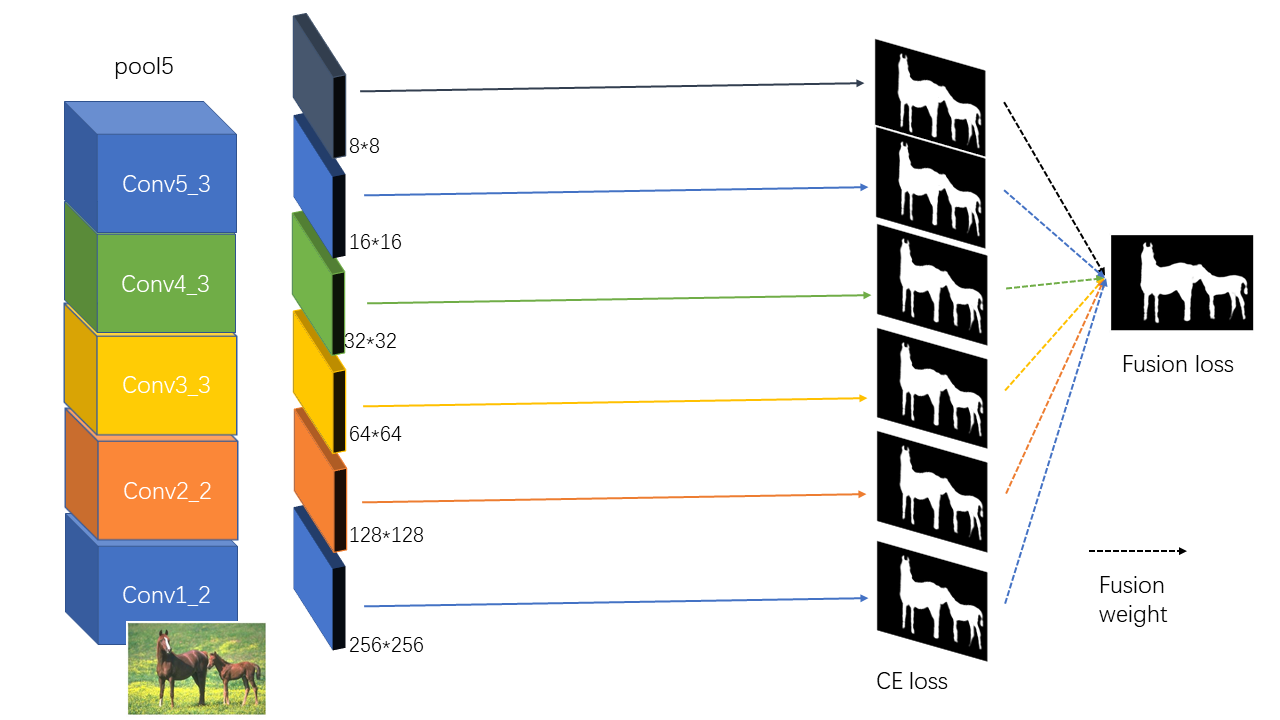
\includegraphics[height=5.0cm,width=9.0cm]{figures/HED.png}
	\caption{\textbf{The Refined HED architecture.}}
\end{figure}

Moreover, it is obvious that these side outputs represent different levels of features. The deeper side outputs contain more semantic features while the shallower side outputs contain more boundary information. So a combination of these side outputs yield better results. Therefore, as is suggested in\cite{hou2017deeply}, we add substantial short connections in the network architecture. The final backbone of our network is presented as follows.
\begin{figure}[!htbp]
	\centering
	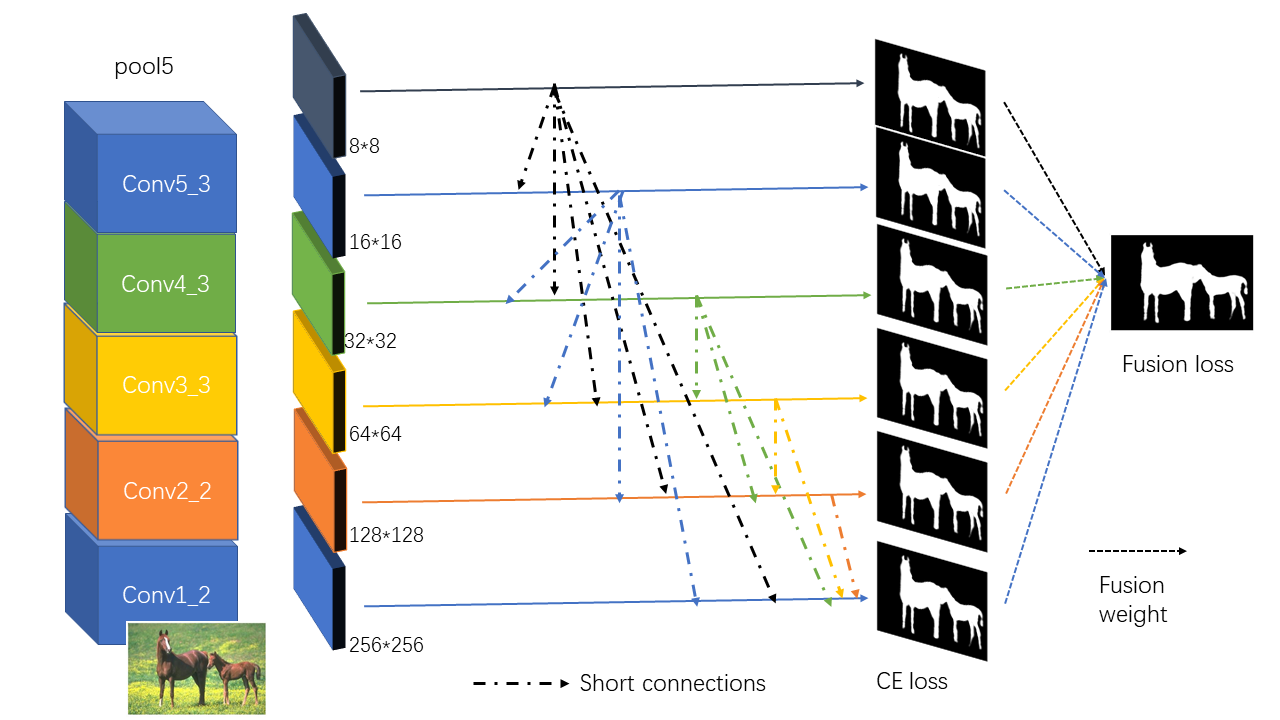
\includegraphics[height=5.0cm,width=9.0cm]{figures/HED_DSS.png}
	\caption{\textbf{The Refined HED architecture with short connections.}}
\end{figure}


\subsection{Robust Background Detection}
We select RBD\cite{zhu2014saliency} as our handcrafted saliency detection model since it is one of the best handcrafted saliency detection methods and it takes both spatial layout and background weighted contrast into consideration.

First of all, we can abstract the image as a set of nearly regular super pixels using the SLIC method. Then we create an undirected weighted graph connect all the adjacent super pixels and assign the distance between two superpixels as the Euclidean distance between their average colors in the CIE-Lab color space. Based on the distance between different pairs of super pixels we then can get the spanning area of a super pixel which includes the super pixels that can be reached with a limited length of edges in the weighted graph. For a spanning area, we can calculate how this area is connected with the image’s boudaries.

In spatial layout, RBD is developed based on the statistical observation that our target salient objects and background regions in most of the images are very different in their spatial layout. The salient object regions are much less connected with the image’s boundaries and meanwhile the background regions are very connected with the images’ boundaries. So, we can define the Background connectivity to represent how much one given region is connected with the image boundaries:

\begin{equation}
\operatorname { BndCon } ( p ) = \frac { \operatorname { Len } _ { b n d } ( p ) } { \sqrt { \operatorname { Arca } ( p ) } }
\end{equation}

In this formula $BndCon(p)$ means the boundary connectivity and it is obvious that super pixel with higher boundary connectivity is more likely to be in the background in the original image. Thus, we can further define the background probability $\omega_i^bg$ which is close to 1 when boundary connectivity is large and close to 0 when it is small.

Furthermore, the background weighted contrast is introduced to compute saliency for a given super pixel p which is defined as:
\begin{equation}
w C t r ( p ) = \sum _ { i = 1 } ^ { N } d _ { a p p } \left( p , p _ { i } \right) w _ { s p a } \left( p , p _ { i } \right) w _ { i } ^ { b g }
\end{equation}

$W_{spa} (p, pi)$ represents the spatial distance between the center of p and pi. From this formula the salient object regions get high  $\omega_i^{bg}$ from the background regions and thus their contrast is enhanced while the background regions receive small $\omega_i^{bg}$ from the salient object regions and thus their contrast is attenuated. So, this operation effectively enlarges the contrast differences between the object and the background regions. 

Finally, we fuse our handcrafted features with our side outputs to let the handcrafted prior to guide our model.
\begin{figure}[!htbp]
	\centering
	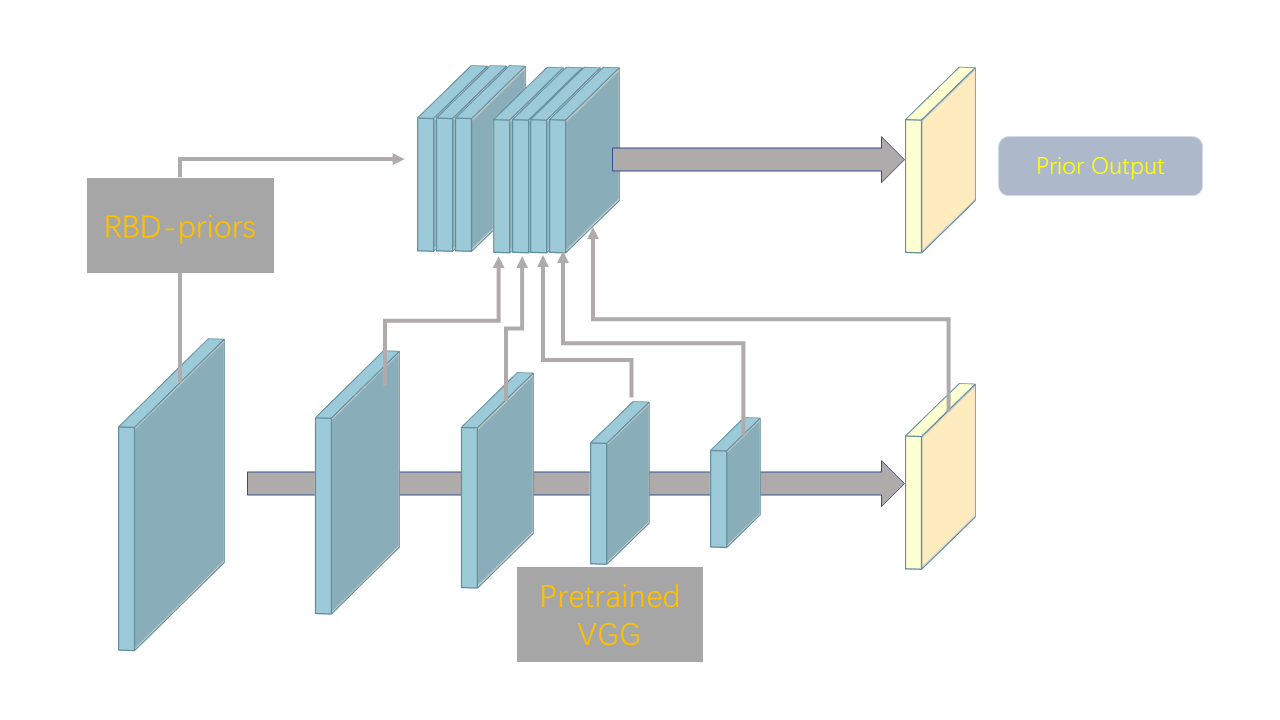
\includegraphics[height=6.0cm,width=9.5cm]{figures/RBD_net.png}
	\caption{\textbf{The RBD network architecture.} The side-outputs are concated and processed by convolutional layers.}
\end{figure}
\subsection{Boundary Refinement}

Our HED based architecture with short connections can aggregate a lot of useful features by combing different layer side-outputs and preserve some low-level details, but a lot of details in the boundary region are still missing. So, in order to recover continuous details for obtaining spatial precision, we have used a local boundary refinement network (BRN)\cite{wang2018detect} to rectify our prediction in boundary regions, which processes as follows.

\begin{figure}[htbp]
	\centering
	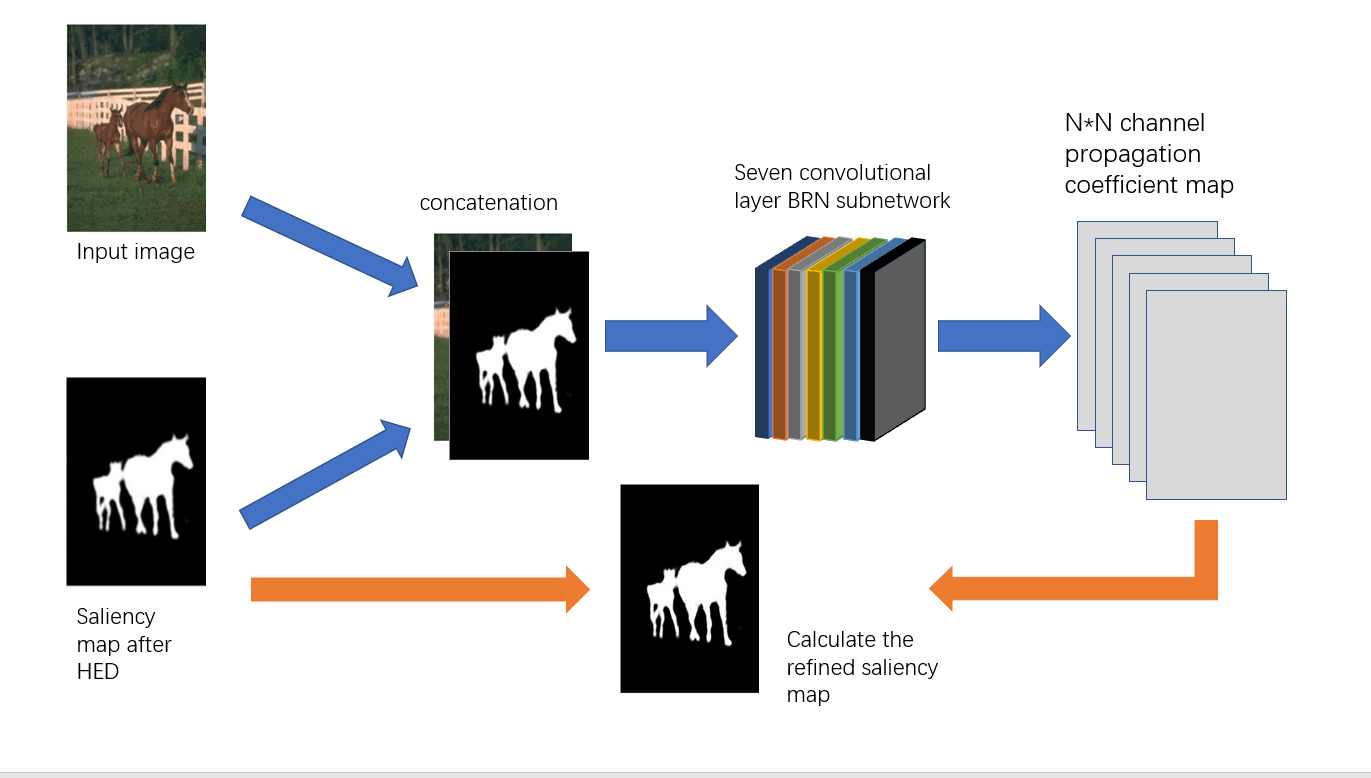
\includegraphics[height=4cm,width=9.5cm]{figures/brn.png}
	\caption{\textbf{The high level structure of BRN.} BRN subnet learns a $n\times n$ channel feature map to extract the features of neighboring pixels.}
\end{figure}

First, we concatenate the saliency map produced by our HED based architecture with the original RGB image and take it as the input of our BRN sub network. For each position in the image, our BRN sub network aims at learning a n*n propagation coefficient map with which local context information can be aggregated to the center pixel and thus we could improve the boundary region.

For position i, BRN will first produce a propagation coefficient vector, which is actually a n$\times$n square. The refinement map at position i can be generated by the multiplied sum of the propagation map and the original saliency map in the neighbors of i.
\begin{equation}
\mathbf { s } _ { i } ^ { \prime } = \sum _ { d = 1 } ^ { n \times n } \mathbf { v } _ { i } ^ { d } \cdot \mathbf { s } _ { i } ^ { d } , d \in 1,2 , \dots , n \times n
\end{equation}

In this formula $V_i^d$ is the coefficient vector of the d-th neighbor at position $i$. $n\times n$ represents the size of pixel $i's$  local neighbors, which we think will have impact on its saliency. $S_i^d$ denotes the prediction vector at location $i$ before the refinement and $S_i^{\prime}$ denotes the vector after the refinement. Each position in BRN has its own different propagation coefficient and it will be learned during the training.

\section{Experiments}
In this Section, we have made substantial experiments to validate the effectiveness of our model.
\subsection{Experimental Setups}
\noindent\textbf{Datasets.}
The MSRA-B dataset contains 5,000 labeled images. We randomly divide these 5,000 images into a 4,000 training set and a 1,000 validation set. Jittering and mirroring are adopted for data augmentation.
The ECSSD dataset contains 1,000 labeled images, and the HKU-IS dataset contains more than 4,000 labeled images. We use both dataset as the test set to verify the generality of our model.\\
\noindent\textbf{Evaluation Protocols}
In our experiments, the performance of our model is mainly evaluated by the $F_\beta$.
\begin{equation}
F _ { \beta } = \frac { \left( 1 + \beta ^ { 2 } \right) \text { Precision } \times \text {Recall} } { \beta ^ { 2 } \times \text { Precision } + \text {Recall} }
\end{equation}
To leverage the importance of precision and recall, $\beta ^2$ is set to $0.3$.
We also use MAE as substantial evaluation metric. $$mae=\frac{N_{pixels\ predicted\ right}}{N_{pixels\ of\ image}}$$
$N_{pixels\ predicted\ right}$ is the number of pixels which are correctly predicted, while $N_{pixels\ of\ image}$ depicts the number of pixels for an image.
\subsection{Implementation Details}
\noindent\textbf{Network Structure for BRN.} 
For BRN subnet, the implementation details are shown in the table below. BRN has 7 convolutional layers and their kernels are 3*3. We add ReLU operations between two convolutional layers to keep nonlinearity. To keep the same resolution between our original input and output feature maps we do not apply any pooling layers. 
In BRN subnet, we learn a matrix of size $K*H*W*25$ as $tmp1$, where $K$ denotes the batch size, and $H,W$ denote the image's height and width respectively.  Then, we concat the last prediction of HED architecture and the original image, pass it through  convolutional layers to form a matrix of the same size $K*H*W*25$ as $tmp2$. Then we use the dot product of $tmp1$ and $tmp2$ to form a new boundary refined feature map. 
\begin{table}[!htbp]
	\centering
	\tablename{ The architecture of BRN subnet}
	\begin{tabular}[I]{cccc}
		\hline
	    Layer & Channel& Kernel size&Bias size\\
		\hline
		1& 64& (K+3)$\times$64$\times$3$\times$3 & 64 \\
		2& 64& 64$\times$64$\times$3$\times$3 & 64 \\
		3& 64& 64$\times$64$\times$3$\times$3 & 64 \\
		4& 64& 64$\times$128$\times$3$\times$3 & 128 \\
		5& 64& 128$\times$128$\times$3$\times$3 & 128 \\
		6& 64& 128$\times$128$\times$3$\times$3 & 128 \\
		7& 64& 128$\times$(n$\times$n)$\times$3$\times$3 & 5$\times$5 \\
		\hline
	\end{tabular}
\end{table} 

\noindent\textbf{Network Structure for RBD.} 
For RBD, we simply concat the RBD output(4-channel) with the original HED side outputs(7-channel). To make sure the original details isn't lost, we also concat the original RGB channels(3-channel) with the side outputs. Therefore, the side output consists of 14 channels. Then, unlike BRN, we use convolutional layers to process the side outputs to get the salient image.

\noindent\textbf{Training Details.}
For training, we use Adam optimizer to accelerate the converge speed. Also, we used pretrained $vgg16$. We adopt learning rate decay strategy,  with the learning rate before epoch $30$ set $5e^{-4}$, and after epoch $30$ $5e^{-5}$. The weight initialization we adopt is Xavier. Both of the networks are trained with a batch size of 32. 
\subsection{Results on Different Datasets}
\noindent\textbf{Learning curve.} The learning curves of both networks are presented as follows. The converge speed is fast, as we have used pre-trained vgg16 in our training.
\begin{figure}[!htbp]
	\centering
	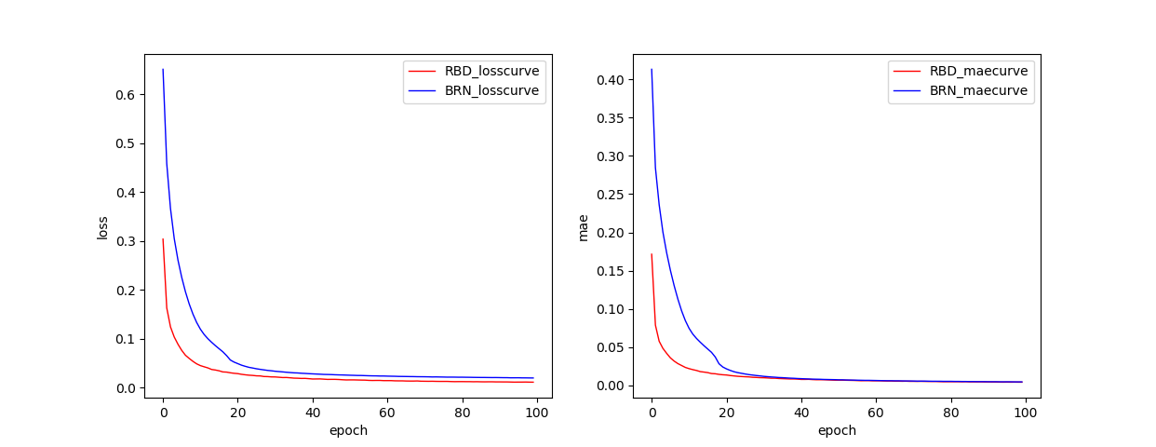
\includegraphics[height=4cm,width=9.5cm]{figures/lrcurve.png}
	\caption{\textbf{The learning curves.}  The converge speed of RBD is relatively higher and the original MAE of RBD is also relatively lower. This is because in RBD approach, saliency prior information is adopted, thus the model already has some learning abilities from the very beginning.}
\end{figure}

\noindent\textbf{Statistic Comparison.} The statistical comparison is presented as follows. From the table, we could observe that in $Fscore$, both of our approaches reached comparable results with the state of art results. And the F-score of our RBD approach is slightly better than the original DSS. 
\begin{table}[!htbp]
	\centering
	\tablename{ F-score of all approaches on different datasets.}
	\begin{tabular}[I]{cccc}
		\hline
		& MSRA-B validation& ECSSD&HKU-IS\\
		\hline
		Original E-HED& 0.9312 & 0.9264 & 0.9295 \\
		E-HED+RBD&\textbf{0.9329}& \textbf{0.9268}& \textbf{0.9305} \\
		E-HED+BRN& 0.9302& 0.9244& 0.9267 \\
		\hline
	\end{tabular}
\end{table}

The substantial MAE metrics is presented as follows. Our BRN approach has a relatively lower MAE than the original network. This is because the BRN focuses on refining boundary, thus more detail is well preserved, which makes the MAE metric lower. 
\begin{table}[!htbp]
	\centering
	\tablename{ MAE of all approaches on different datasets.}
	\begin{tabular}[I]{cccc}
		\hline
		& MSRA-B validation& ECSSD&HKU-IS\\
		\hline
		Original E-HED& 0.0562 & 0.0428 & 0.0441 \\
		E-HED+RBD& 0.0593& 0.0414& 0.0446 \\
		E-HED+BRN& \textbf{0.0548}& \textbf{0.0408}& \textbf{0.0414}\\
		\hline
	\end{tabular}
\end{table}

\noindent\textbf{Sample Results.}Our model performs well in hard cases, both low contrast and multi-object images.
\begin{figure}[!htbp]
	\centering
	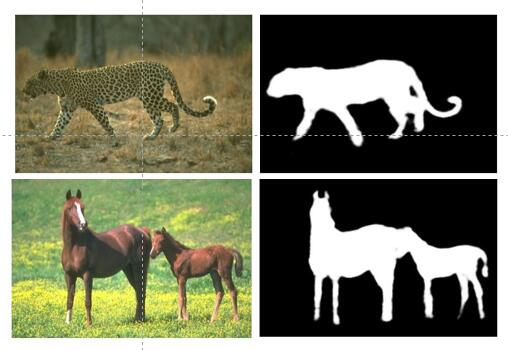
\includegraphics[height=6cm,width=9.0cm]{figures/sample.jpg}
	\caption{\textbf{The sample outcome.}  Both scenes are well predicted, and boundary information are well retained.}
\end{figure}


\section{Conclusion}
In this work, we proposed two different approaches to detect the salient region of an image. Experiments on these two models showed that both of theses approaches reach the state-of-art results, and are efficient in improving the ability to detect salient regions.

\section{Member Contribution}
Here we listed our contributions to this project separately.
\begin{itemize}
    \item \textbf{Bohong Wu 516030910365} Most of the coding work and writing work in the $BRN$ approach. The latex writing of our paper. Some graphs of our paper.
    \item \textbf{Haoqi Zhang 516030910393} Most of the coding work and writing work in the $RBD$ approach. Some graphs of our paper.
\end{itemize}

\bibliographystyle{IEEEtran}
\bibliography{bibtex}


% Can use something like this to put references on a page
% by themselves when using endfloat and the captionsoff option.
\ifCLASSOPTIONcaptionsoff
  \newpage
\fi


\end{document}


